%!Tex Program = xelatex
\documentclass[10pt,a4paper,fleqn]{article}
\usepackage{fontspec, xunicode, xltxtra}
%\usepackage{xeCJK}
\usepackage[slantfont,boldfont]{xeCJK} % 允许斜体和粗体
\usepackage{multirow}
\usepackage{multicol}
\usepackage{titlesec}
\usepackage{enumerate}
\usepackage{booktabs}
\usepackage[table,xcdraw]{xcolor}
\usepackage{float}
\usepackage{geometry}
\usepackage{tikz}
\usepackage{tikz-qtree}
\usepackage{amsmath,amssymb}
\usepackage{extarrows}
\usepackage[colorlinks,linkcolor=black]{hyperref}
\usepackage{zhnumber}
\usepackage{listings}
\usepackage{pdfpages}
\usepackage{dirtree}

\geometry{left=2.5cm,right=2.5cm,top=2cm,bottom=2cm}

%cmd “fc-list :lang=zh-cn”
\defaultfontfeatures{Mapping=tex-text}
\setmainfont{Book Antiqua}   % 英文衬线字体 Times New Roman, Palatino Linotype
\setmonofont{Consolas}   % 英文等宽字体 Monaco
\setsansfont{Consolas} % 英文无衬线字体 Arial, Futura, Optima
\setCJKmainfont{SimSun}   % 设置缺省中文字体
\setCJKmonofont{FangSong}   % 设置等宽字体
\setCJKsansfont{SimHei}   % 设置无衬线字体 Microsoft YaHei

\newfontfamily\timesroman{Times New Roman}
\newfontfamily\consolas{Consolas}

\newfontfamily\ensong{SimSun}
\newfontfamily\enhei{SimHei}
\newfontfamily\enyahei{Microsoft YaHei}
\newfontfamily\palatino{Palatino Linotype}
\newfontfamily\nimbus{Nimbus Sans L}
\newfontfamily\enkai{KaiTi}
\newfontfamily\enfangsong{FangSong}
\newfontfamily\enstzhsong{STZhongsong}
\newfontfamily\enstsong{STSong}

\setCJKfamilyfont{song}{SimSun}
\newcommand{\song}{\CJKfamily{song}}
\setCJKfamilyfont{heiti}{SimHei}
\newcommand{\heiti}{\CJKfamily{heiti}\enhei}
\setCJKfamilyfont{yahei}{Microsoft YaHei}
\newcommand{\yahei}{\CJKfamily{yahei}\enyahei}
\setCJKfamilyfont{kaiti}{KaiTi}
\newcommand{\kaiti}{\CJKfamily{kaiti}\enkai}
\setCJKfamilyfont{fangsong}{FangSong}
\newcommand{\fangsong}{\CJKfamily{fangsong}\enfangsong}
\setCJKfamilyfont{stzhsong}{STZhongsong}
\newcommand{\stzhsong}{\CJKfamily{stzhsong}\enstzhsong}
\setCJKfamilyfont{stsong}{STSong}
\newcommand{\stsong}{\CJKfamily{stsong}\enstsong}

\XeTeXlinebreaklocale "zh"
\XeTeXlinebreakskip = 0pt plus 1pt minus 0.1pt

%------------------------------标题名称中文化-----------------------------%
\renewcommand\abstractname{\heiti 摘\ 要}
\renewcommand\refname{\scriptsize 参考文献}
\renewcommand\figurename{\scriptsize 图}
\renewcommand\tablename{\scriptsize 表}

%\titlespacing*{\chapter} {0pt}{50pt}{40pt}
%\titlespacing*{\section} {0pt}{3.5ex plus 1ex minus .2ex}{2.3ex plus .2ex}
%\titlespacing*{\subsection} {0pt}{3.25ex plus 1ex minus .2ex}{1.5ex plus .2ex}
%\titlespacing*{\subsubsection}{0pt}{3.25ex plus 1ex minus .2ex}{1.5ex plus .2ex}
%\titlespacing*{\paragraph} {0pt}{3.25ex plus 1ex minus .2ex}{1em}
%\titlespacing*{\subparagraph} {\parindent}{3.25ex plus 1ex minus .2ex}{1em}

\titleformat{\section}{\bf\song}{\zhnumber{\thesection}、}{0em}{}
\titleformat{\subsection}{\bf\song}{\thesubsection}{0.5em}{}

%\setlength{\baselineskip}{1em}
\setlength{\parindent}{2em}
\setlength{\parskip}{0.2\baselineskip}
\setlength{\abovedisplayskip}{0.5pt}
\setlength{\belowdisplayskip}{0.5pt}

\newcommand{\hangpar}{\par\noindent\hangafter=1\setlength{\hangindent}{2em}}

\aboverulesep=0pt
\belowrulesep=0pt

\lstset{
    language=verilog,
    basicstyle=\small,
    numbers=left,
    numberstyle=\small,
    stepnumber=1,
    numbersep=5pt,
    backgroundcolor=\color{white},
    %keywordstyle=\color{keywordcolor}\bfseries, %\underbar,
    keywordstyle=\color{blue}\bfseries,
    morekeywords={*,\$write},
    identifierstyle=\small,
    showspaces=false,
    showstringspaces=false,
    showtabs=false,
    tabsize=4,
    frame=single,
    commentstyle=\color{olive} \textit,
    stringstyle=\ttfamily,
    showstringspaces=false,
    captionpos=b,
    breaklines=true,
    breakatwhitespace=true,
  }

\lstdefinelanguage{Assembler} {
  numberblanklines=false,
  keywordstyle=\color{blue}\bfseries,
  morekeywords={nop,halt,load,ld,store,str,ldih,mov,
  add,addi,addc,sub,subc,cmp,
  and,or,xor,not,sl,sll,sla,srl,sra,
  j,jump,jmpr,jr,bz,bnz,bn,bnn,bc,bnc},
  morecomment=[l]{\#},
}

\begin{document}
  \begin{center}
  \stzhsong
  \LARGE{中山大学本科生实验报告}\\[10pt]
  \Large{(2016学年春季学期)} \\[20pt]
  \end{center}
  \begin{flushleft}
    \stsong
    课程名称:嵌入式系统案例分析与设计
    \hspace{3em}
    任课教师:  {\bf 王军}
    \hspace{3em}
    助教:杨涵铄
    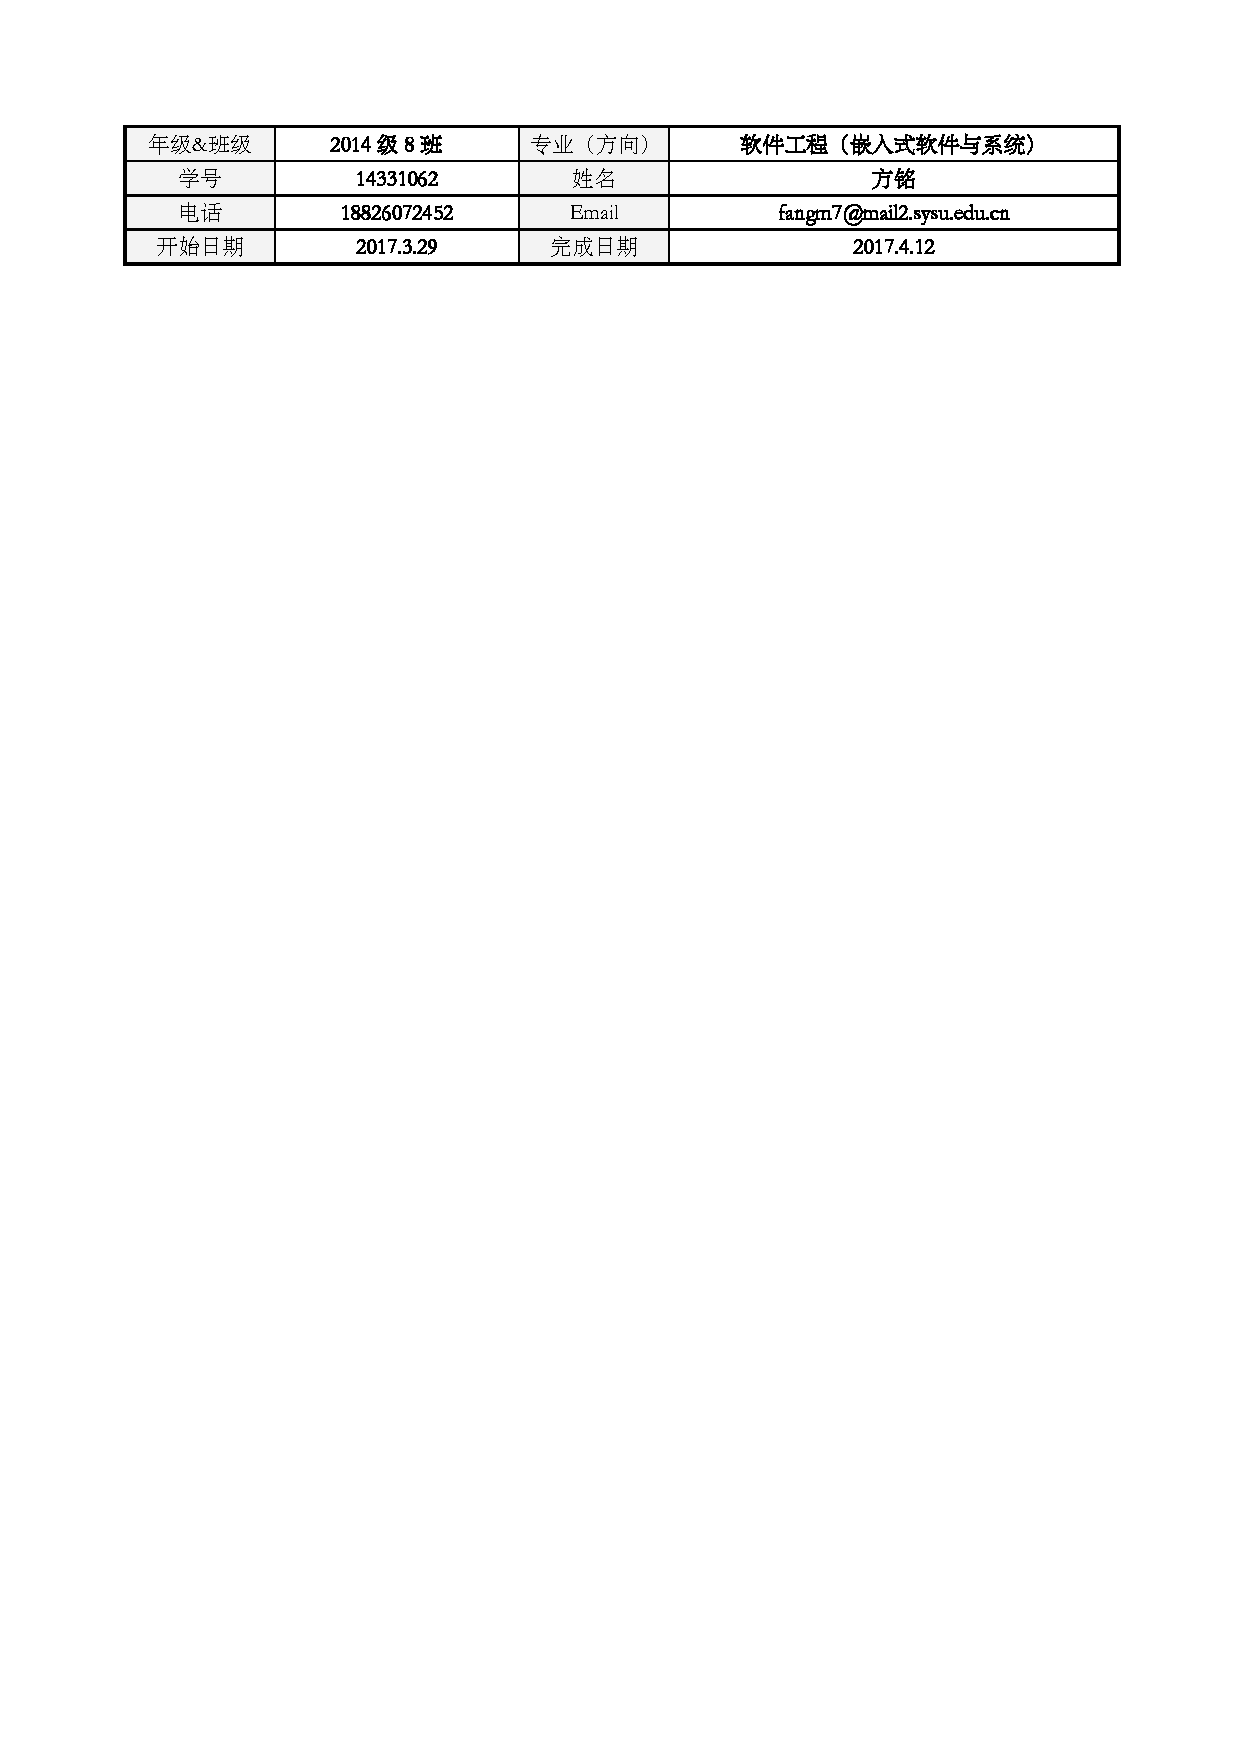
\includegraphics[width=\textwidth]{figure/info.pdf}
  \end{flushleft}

  {\noindent\bf\kaiti 实验题目:\palatino Case 1:Pipeline Processor% with Hazard
  }

  \section{实验目的}
\begin{enumerate}
  \item 认识和掌握基于精简指令集(RISC)的简单流水线处理器原理及其设计方法;
  \item 掌握流水线处理器的verilog代码实现方法及其测试;
  \item 分析指令集,明确指令功能、指令在CPU中执行各阶段中的行为;
  %\item 编写测试用的汇编指令,并将汇编指令转换为二进制的指令编码,并且 加载到处理器中的指令存储器中。
  \item 掌握较复杂的设计在FPGA实验板上的综合实现,并通过开发板上的led或数码管显示执行效果。
\end{enumerate}

  \section{实验内容}
  \subsection*{实验步骤}
  \begin{enumerate}
    \item 分析并设计处理器的数据通路和控制通路。
    \item 编写设计代码并编译。
    \item 软件仿真。
    \item 进行硬件配置。
  \end{enumerate}
  \subsection*{实验要求}
\begin{description}
  \item[·] RISC CPU
  \item[·] Data path 16b
  \item[·] Data memory -$2^8\times16$b
  \item[·] Size of operation set -$2^5$
  \item[·] General register -$8\times16$b
  \item[·] Flags -NF,ZF,CF
  \item[·] Control -clock, reset, enable, start
  \item[·] Testing -4 bit selection for 16 bit output
\end{description}
  \subsection*{实验原理}
类似于RISC体系架构依据流水线结构设计,每条指令就被分成五个流水阶段,并且每个阶段占用固定的时间,即一个时钟周期。

\par 处理器在设计时,将处理器的执行阶段划分为以下五个阶段:
\begin{description}
  \item[IF] Instruction Fetch,取指。从指令缓存(I-Cache)中获取下一条指令。
  \item[ID] Instruction Decode(Read Register),译码(读寄存器)。翻译指令,识别操作码和操作数,从寄存器堆中读取数据到ALU输入寄存器。
  \item[EX] Execute,执行(算术/逻辑运算)。在一个时钟周期内,完成算术或逻辑操作。注意,浮点算术运算和整数乘除运算不能在一个时钟周期内完成。
  \item[MEM] Memory Access,内存数据读或者写。在该阶段,指令可以从数据缓存(D-Cache)中读/写内存变量。平均来说,大约四分之三的指令在这一阶段没有执行任何操作,为每条指令分配这个阶段是为了保证同一时刻不会有两条指令都访问数据缓存。
  \item[WB] Write Back,写回。操作完成后,将计算结果从ALU输出寄存器写回到通用寄存器中
\end{description}
\subsubsection*{实验假设}
\begin{enumerate}
  \item 本实验不实现自启动的控制电路,也不提供进程切换所需引脚,不实现进程切换,读、写、内部寄存器的功能。
  \item 本实验认为指令和数据有两个独立的缓存,同时读写不会有冲突。
  \item 本实验认为指令地址和数据地址均已经被映射到缓存(cache)中,读写可在一个时钟周期内完成,从而满足流水线的要求。
  \item 本实验暂时未实现自动处理冒险(hazard),冒险的解决方法依赖于通过软件层面汇编器的在会导致冒险的指令前插入一定数量的nop指令。
  \item 本实验运行的时钟频率较低,是为了在实验板(Xlinx$^{\textregistered}$ Spartan6 XC6LX16-CS324)上观察调试。可以在实验板上正常工作的最大时钟频率暂未测定。
\end{enumerate}
\begin{figure}[H]
  \centering
  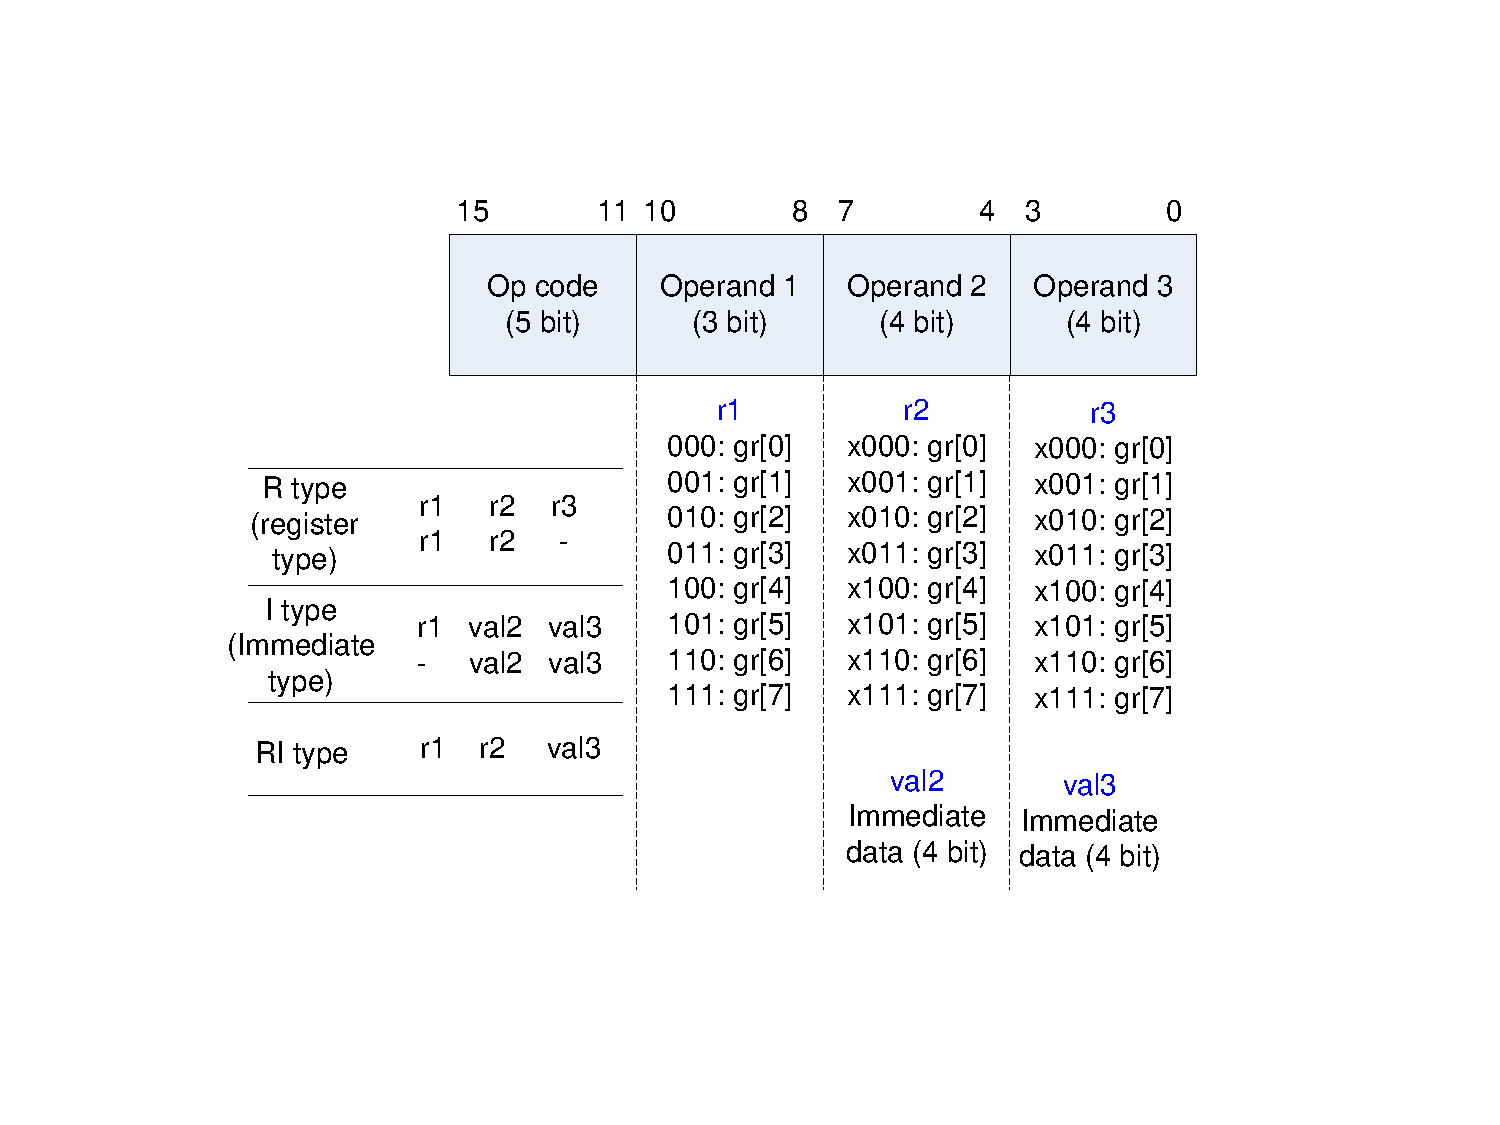
\includegraphics[width=0.6\textwidth]{figure/OpField.pdf}
  \caption{Operation Field}
\end{figure}

\begin{table}[H]
  \rowcolors{2}{blue!20}{blue!10}
  \def\tc{\color{blue}}
  \centering
  \begin{tabular}{llllll}
%    \foreach \text in{mnemonic,operand1,operand2,operand3,op code} {
%     \color{blue}\text &
%    }
%    \color{blue}operation \\
    \tc mnemonic&\tc operand1&\tc operand2&\tc operand3&\tc op code&\tc operation \\
     NOP& & & &00000&no operation\\
     HALT& & & &00001&halt\\
     LOAD&r1&r2&val3&00010&gr[r1]<-m[r2+val]\\
     STORE&r1&r2&val3&00011&m[r2+val]<-r1\\
     LDIH&r1&val2&val3&10000&r1<-r1+\{val2,val3,8'b0\}\\
     MOV&r1&val2&val3&10100&r1<-\{val2,val3\}\\
     ADD&r1&r2&r3&01000&r1<-r2+r3\\
     ADDI&r1&val2&val3&01001&r1<-r1+\{val2,val3\}\\
     ADDC&r1&r2&r3&10001&r1<-r2+r3+CF\\
     SUB&r1&r2&r3&01010&r1<-r2-r3\\
     SUBI&r1&val2&val3&01011&r1<-r1-\{val2,val3\}\\
     SUBC&r1&r2&r3&10010&r1<-r2-r3+CF\\
     CMP& &r2&r3&01100&r2-r3;set CD,ZF and NF\\
  \end{tabular}
  \caption{Data transfer \& Arithmetic Operation}
\end{table}

\begin{table}[H]
  \rowcolors{2}{blue!20}{blue!10}
  \def\tc{\color{blue}}
  \centering
  \begin{tabular}{llllll}
    \tc mnemonic&\tc operand1&\tc operand2&\tc operand3&\tc op code&\tc operation \\
     AND&r1&r2&r3&01101&r1 <- r2 and r3\\
     OR&r1&r2&r3&01110&r1 <- r2 or r3\\
     XOR&r1&r2&r3&01111&r1 <- r2 xor r3\\
     NOT&r1&r2& &10011&r1<- ~r1\\
     SL(SLL/SLA)&r1&r2&val3&00100&r1 <- r2 << val3\\
     SRL&r1&r2&val3&00101&r1 <- r2 >> val3 (logically)\\
     SRA&r1&r2&val3&00110&r1 <- r2 >> val3 (arithmetically)\\
  \end{tabular}
  \caption{Logical / shift}
\end{table}

\begin{table}[H]
  \rowcolors{2}{blue!20}{blue!10}
  \def\tc{\color{blue}}
  \centering
  \begin{tabular}{llllll}
    \tc mnemonic&\tc operand1&\tc operand2&\tc operand3&\tc op code&\tc operation \\
     JUMP& &val2&val3&11000&jump to \{val2,val3\}\\
     JMPR&r1&val2&val3&11001&jump to r1+\{val2,val3\}\\
     BZ&r1&val2&val3&11010&if ZF=1 branch to r1+\{val2,val3\}\\
     BNZ&r1&val2&val3&11011&if ZF=0 branch to r1+\{val2,val3\}\\
     BN&r1&val2&val3&11100&if NF=1 branch to r1+\{val2,val3\}\\
     BNN&r1&val2&val3&11101&if NF=0 branch to r1+\{val2,val3\}\\
     BC&r1&val2&val3&11110&if CF=1 branch to r1+\{val2,val3\}\\
     BNC&r1&val2&val3&11111&if CF=0 branch to r1+\{val2,val3\}\\
  \end{tabular}
  \caption{Control}
\end{table}
\begin{figure}[H]
  \centering
  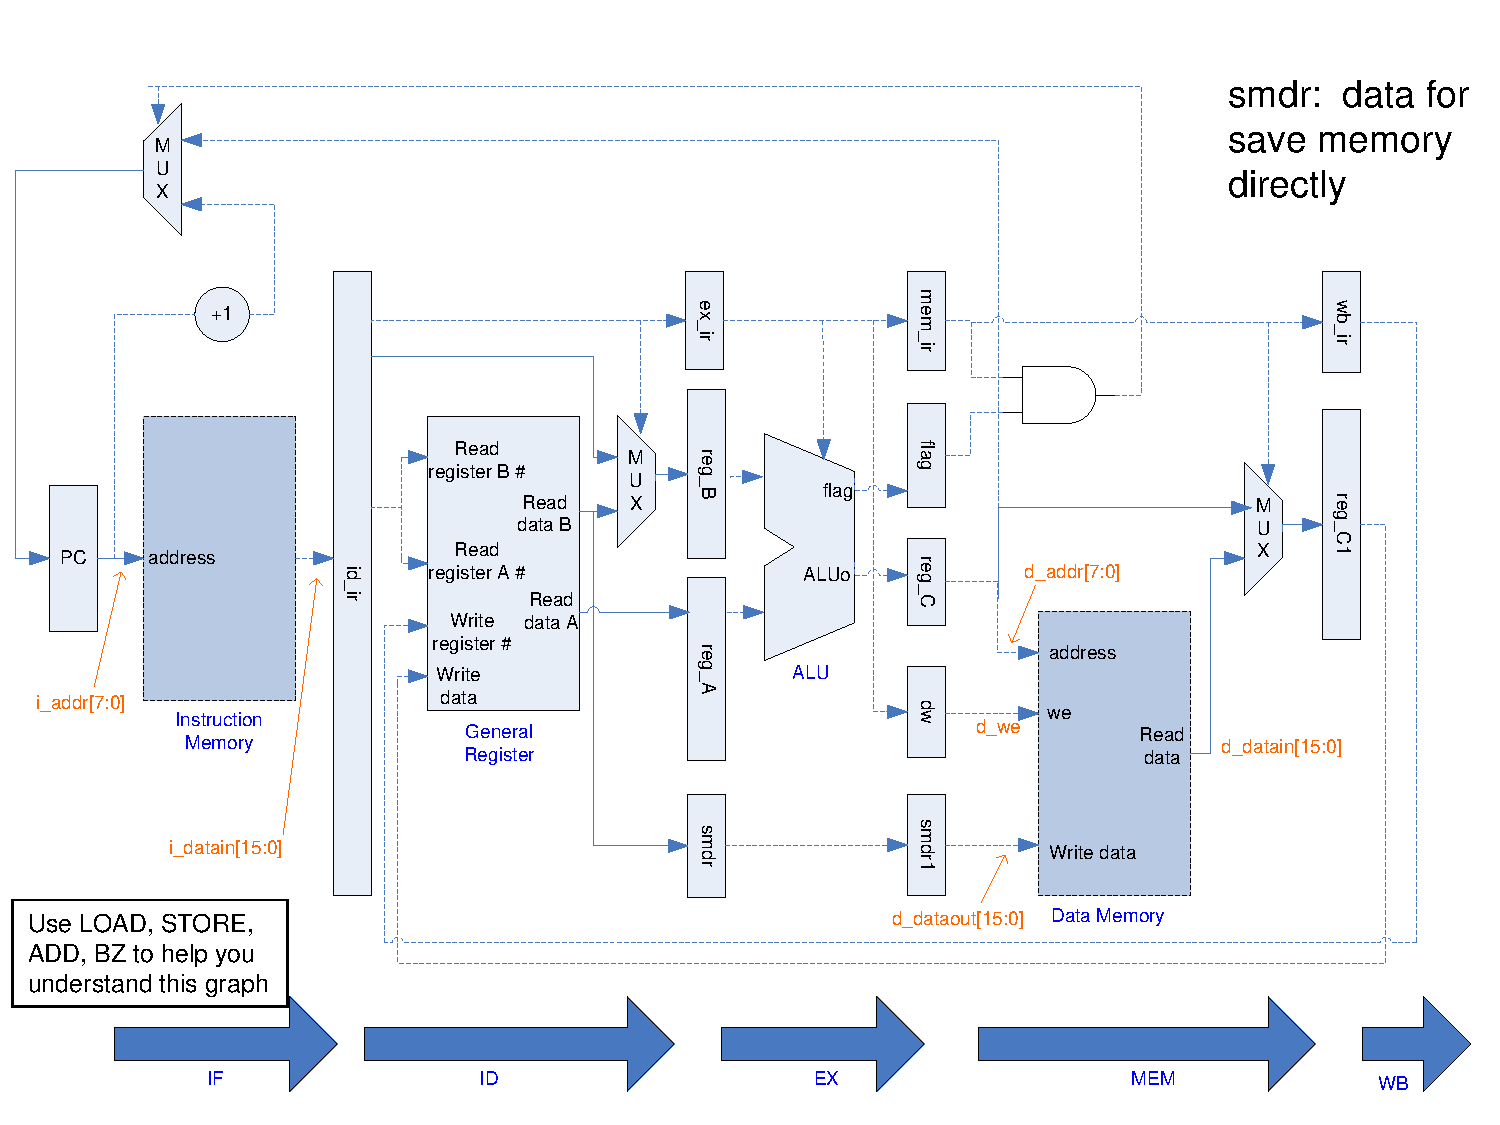
\includegraphics[width=\textwidth]{figure/blockdiagram.pdf}
  \caption{Block Diagram}
\end{figure}
\begin{figure}[H]
  \centering
  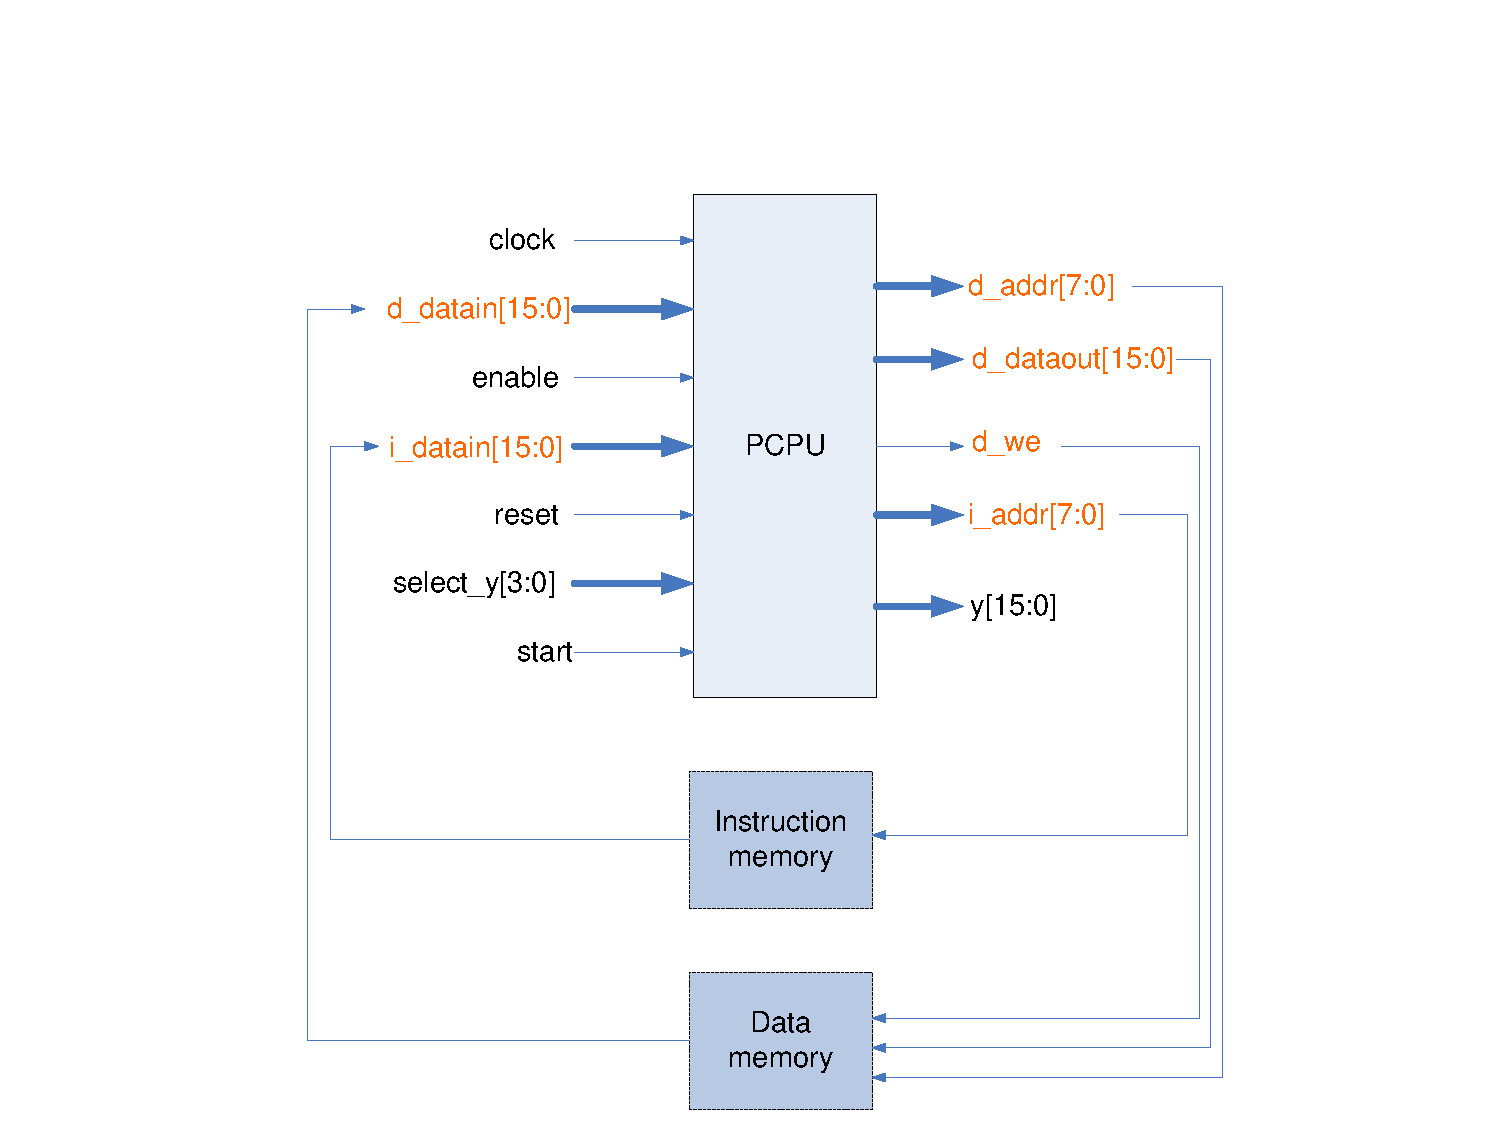
\includegraphics[width=0.7\textwidth]{figure/topview.pdf}
  \caption{Top View}
\end{figure}


  \section{实验结果}
\subsection{综合的RTL电路图}
顶层模块、PCPU模块的 RTL图见附录。\\
时钟分屏、数码管译码模块省略。
\par 手动时钟模块的RTL图如下。
\begin{figure}[H]
  \hspace{-1.5cm}
  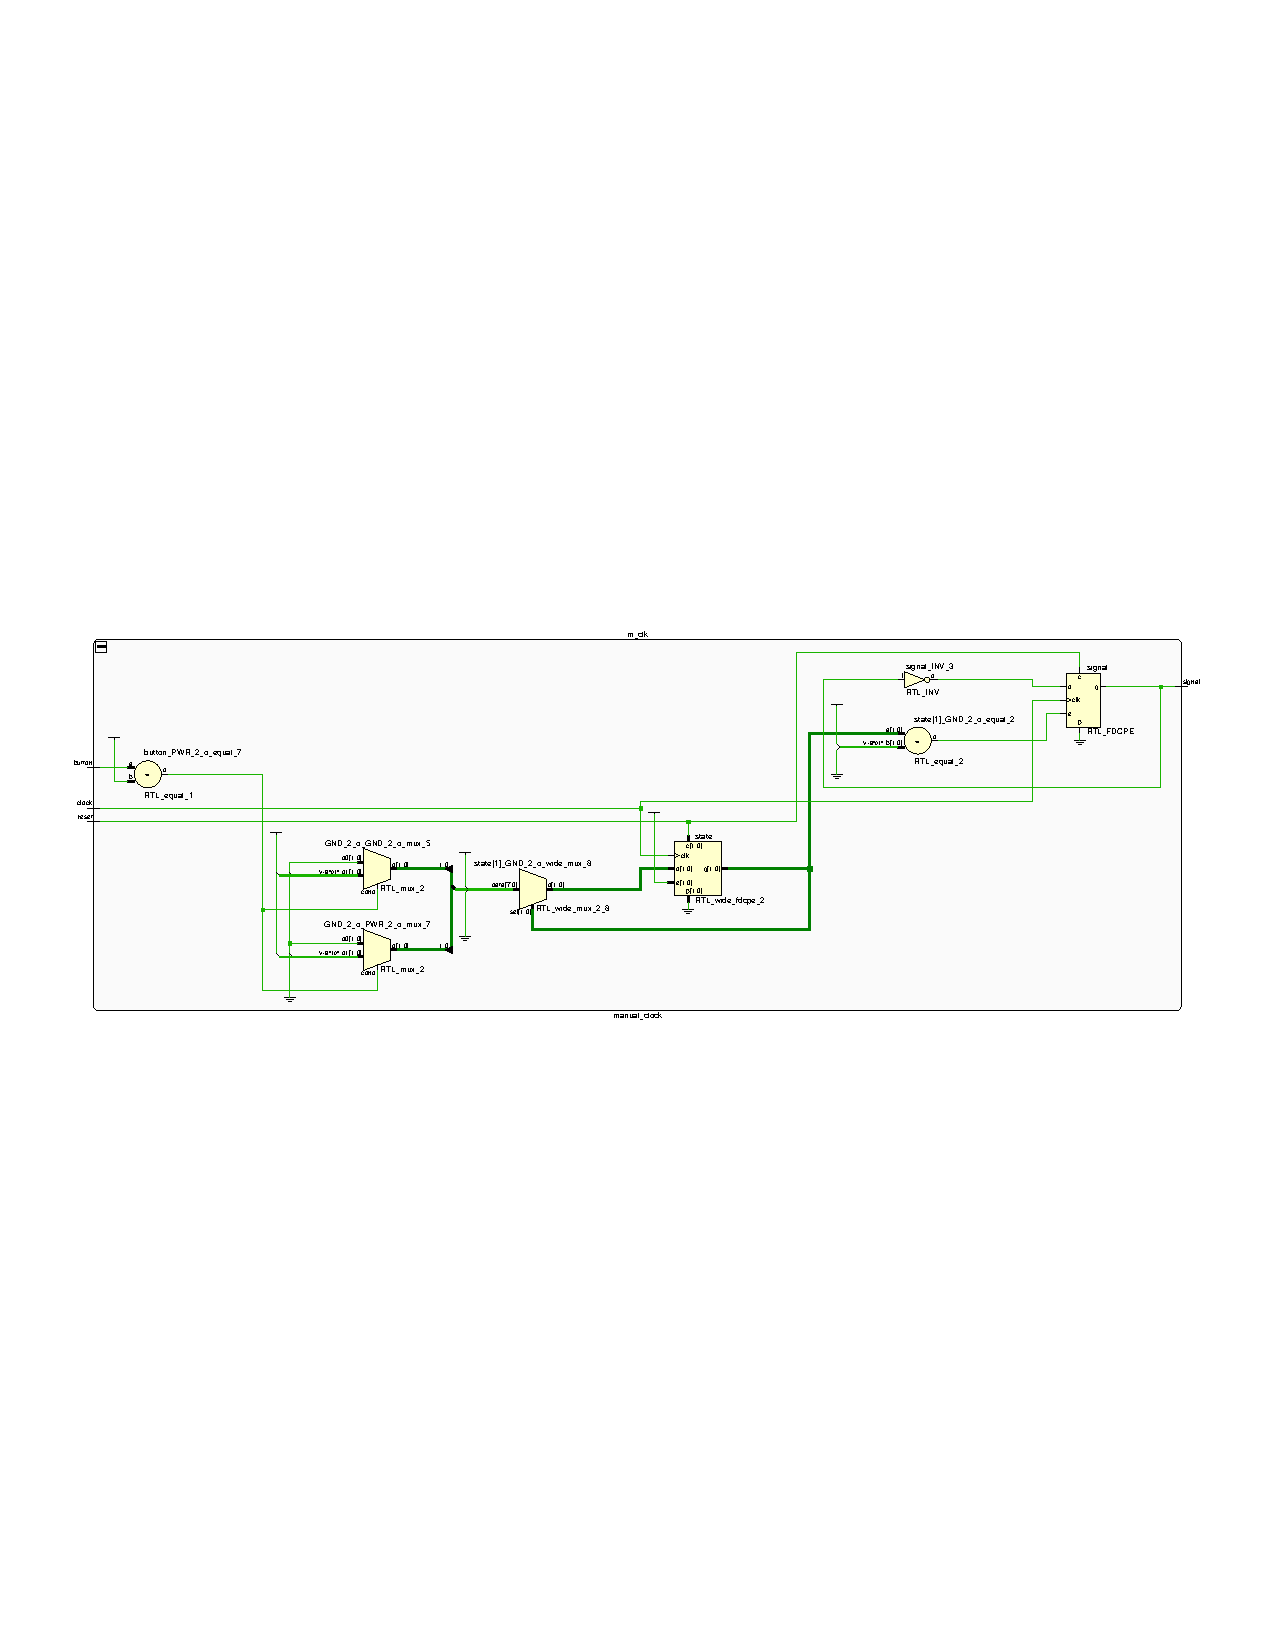
\includegraphics[width=1.2\textwidth]{figure/manualclock.pdf}
  \caption{手动时钟模块的RTL图(Xilinx PlanAhead 14.7导出)}
\end{figure}
\par 经验证,各模块综合出的RTL图与原理图基本一致,综合正确。

\subsection{texture simulation}

\begin{figure}[H]
  \centering
  \begin{minipage}{0.3\textwidth}
    汇编代码 code.asm
    \lstinputlisting[language=Assembler,firstnumber=0]{code/code.asm}
  \end{minipage}
  \hspace{0.5cm}
  \begin{minipage}{0.6\textwidth}
    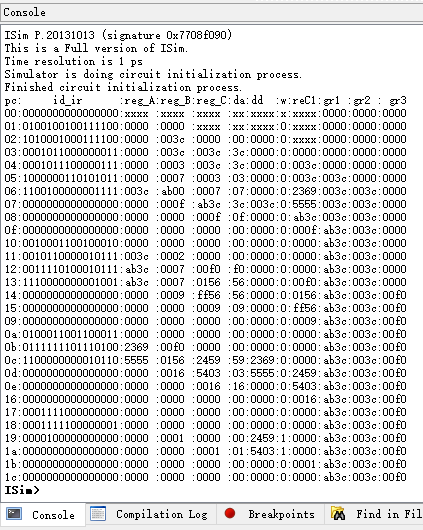
\includegraphics[width=\textwidth]{figure/texture.png}
    \caption{Simulation results}
  \end{minipage}
\end{figure}
经分析对比,pc寄存器和其他寄存器结果、控制信合结果均正确,仿真测试通过。
\subsection{开发板的显示效果}
管脚约束定义见附录。烧入以上程序,全部运行结束后,通用寄存器的结果显示如下:
\begin{figure}[H]
  \centering
  \foreach \n in {0,...,3} {
    \begin{minipage}{0.45\textwidth}
      \includegraphics[width=\textwidth]{figure/gr/\n.jpg}
    \end{minipage}
  }
\end{figure}
\begin{figure}[H]
  \centering
  \foreach \n in {4,...,7} {
    \begin{minipage}{0.45\textwidth}
      \includegraphics[width=\textwidth]{figure/gr/\n.jpg}
    \end{minipage}
  }
  \caption{通用寄存器gr[0:7]的最终结果}
\end{figure}

 \section{实验感想}
   \setlength{\parskip}{0.5\baselineskip}
   \par 本次实验初步实现了一个基于精简指令集的流水线CPU,进一步提高了我设计并实现较复杂硬件系统的能力。
   \par 我原先计划先译码得到各个阶段的控制信号,再对控制信号进行移位,从而并发地控制各级流水单元。后来参考了老师给出的设计图,发现对指令进行移位保存也能实现,而且不容易出错,更适合高级硬件设计语言来描述。虽然理论上,前者消耗的寄存器,门电路会更少,但是通过ISE实现时,还有着一些时间、面积、功耗的约束影响,ISE在特定的约束条件下,对原始的verilog代码优化后,只要在语言描述上是等价的,那么综合出的设计就是几乎一样的,因此我还是认同了第二种方案。虽然类似于smdr,smdr1这种寄存器的声明,看似耗费的资源较多,但实际上,是会被优化掉的。
   \par 以往设计的CPU的经验在本次实验中也得到的了应用,即尽可能少的增加if条件判断,对一些赋不赋值均可的寄存器,如果能减少条件判断,就应该赋值,减少寄存器写使能信号的组合逻辑的复杂度。某些指令与ALU无关,与读写内存无关,只要控制好读写使能信号,就不必要对的这些寄存器清零。
   \par 本次实验基本上没有用到新的知识点,但对逻辑左移右移和算术左移右移之间的区别,以及加减法进位借位的实现不是很有把握,为了减少以后的测试复杂性,我还是事先新建了测试文件,先实现了这些运算的功能,仿真成功后,再写入到PCPU模块去。经过预先测试,发现算术右移一定要声明为signed类型或者通过\$signed()系统函数进行强制类型转换才能实现,否则右移补零和逻辑右移一样。
   \par 经过实验验证并结合我的分析,我认为:使用always @* 语句生成组合电路时,不完整的条件语句会导致latch,但是always @(posedge clk)结合非阻塞赋值 <= 生成的触发器可以没有完整的条件分支。因为这些语句生成的是触发器,分支中赋值的语句的右值作为数据选择器的输入,判断条件通过编码变成一个个选择信号,如果有不完整的条件分支就需要为触发器加一个使能端,为以上条件使能;如果条件分支完整,那么这个触发器不需要使能端,或者令使能端一直处于使能状态。本实验中,我在设计触发器部分时,由于需要保持原来的数据,条件分支没有写完整,但最后也没有任何warning提示生成了latch;相反在利用always @*设计的组合逻辑部分,如果在某个条件分支里写了类似 x = x这样的代码,即使条件完整,也会有warning提示生成了latch。
   \par 原以为这次实验仿真效果可能会与综合效果不同,所以我比较谨慎地消除了几乎所有的warning。初步设计完后,我直接在板子上综合了,综合出现的问题,后来一仿真也有同样的问题。因此,如果设计代码在综合后没有大量warning的话,仿真的效果是和综合效果基本是同步的,仿真的结果是可以信赖的。
   \par 实验中使用了Core\_Gernerate 生成了IP,使用了coe文件初始化内存。根据我的理解,IP可以生成一些高级模块的代码,从而进一步完成更加复杂的设计,比如生成一些浮点运算的模块。这可以帮助设计人员减少开发周期,更加快速地设计一些硬件系统。
%  \newpage
  \appendix
  \titleformat{\section}{\bf\song}{\thesection}{1em}{}
  \newpage
\section*{附录}
  \par 部分图片受版面限制,打印后可能导致阅读不便。此份报告使用的图片均为矢量图,可浏览电子版文档放大后阅读。
  本次实验的项目文件、汇编指令解释器及coe生成程序及实验报告可访问
  \url{https://github.com/SimonFang1/Pipeline-RISC-CPU/}查看。
  %\renewcommand{\appendixname}{Appendix~\Alph{section}}
\section{较复杂的RTL电路图}
\begin{figure}[H]
  \centering
  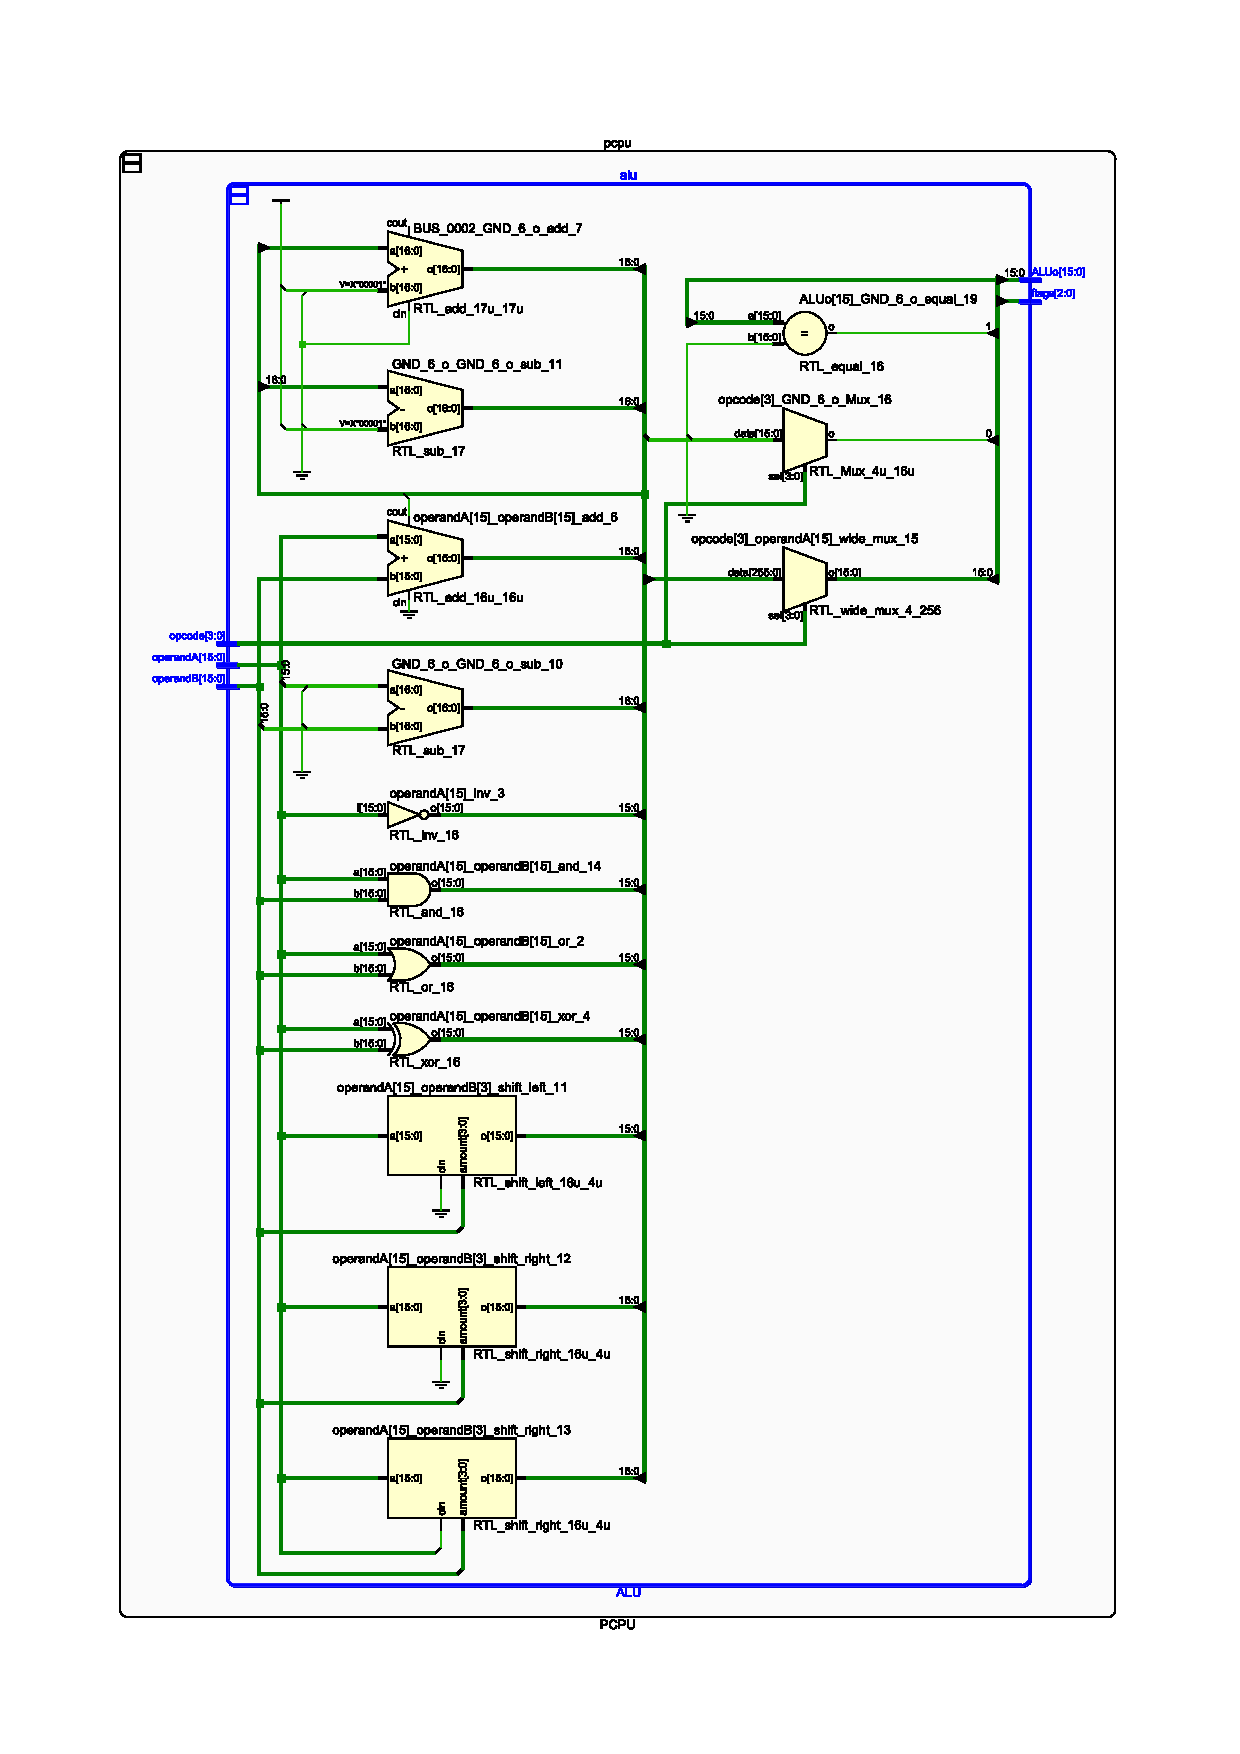
\includegraphics[width=0.85\textwidth]{figure/aluex.pdf}
  \caption{ALU模块的RTL图(Xilinx PlanAhead 14.7导出)}
\end{figure}
\newpage
\thispagestyle{empty}
\begin{figure}[H]
  \centering
  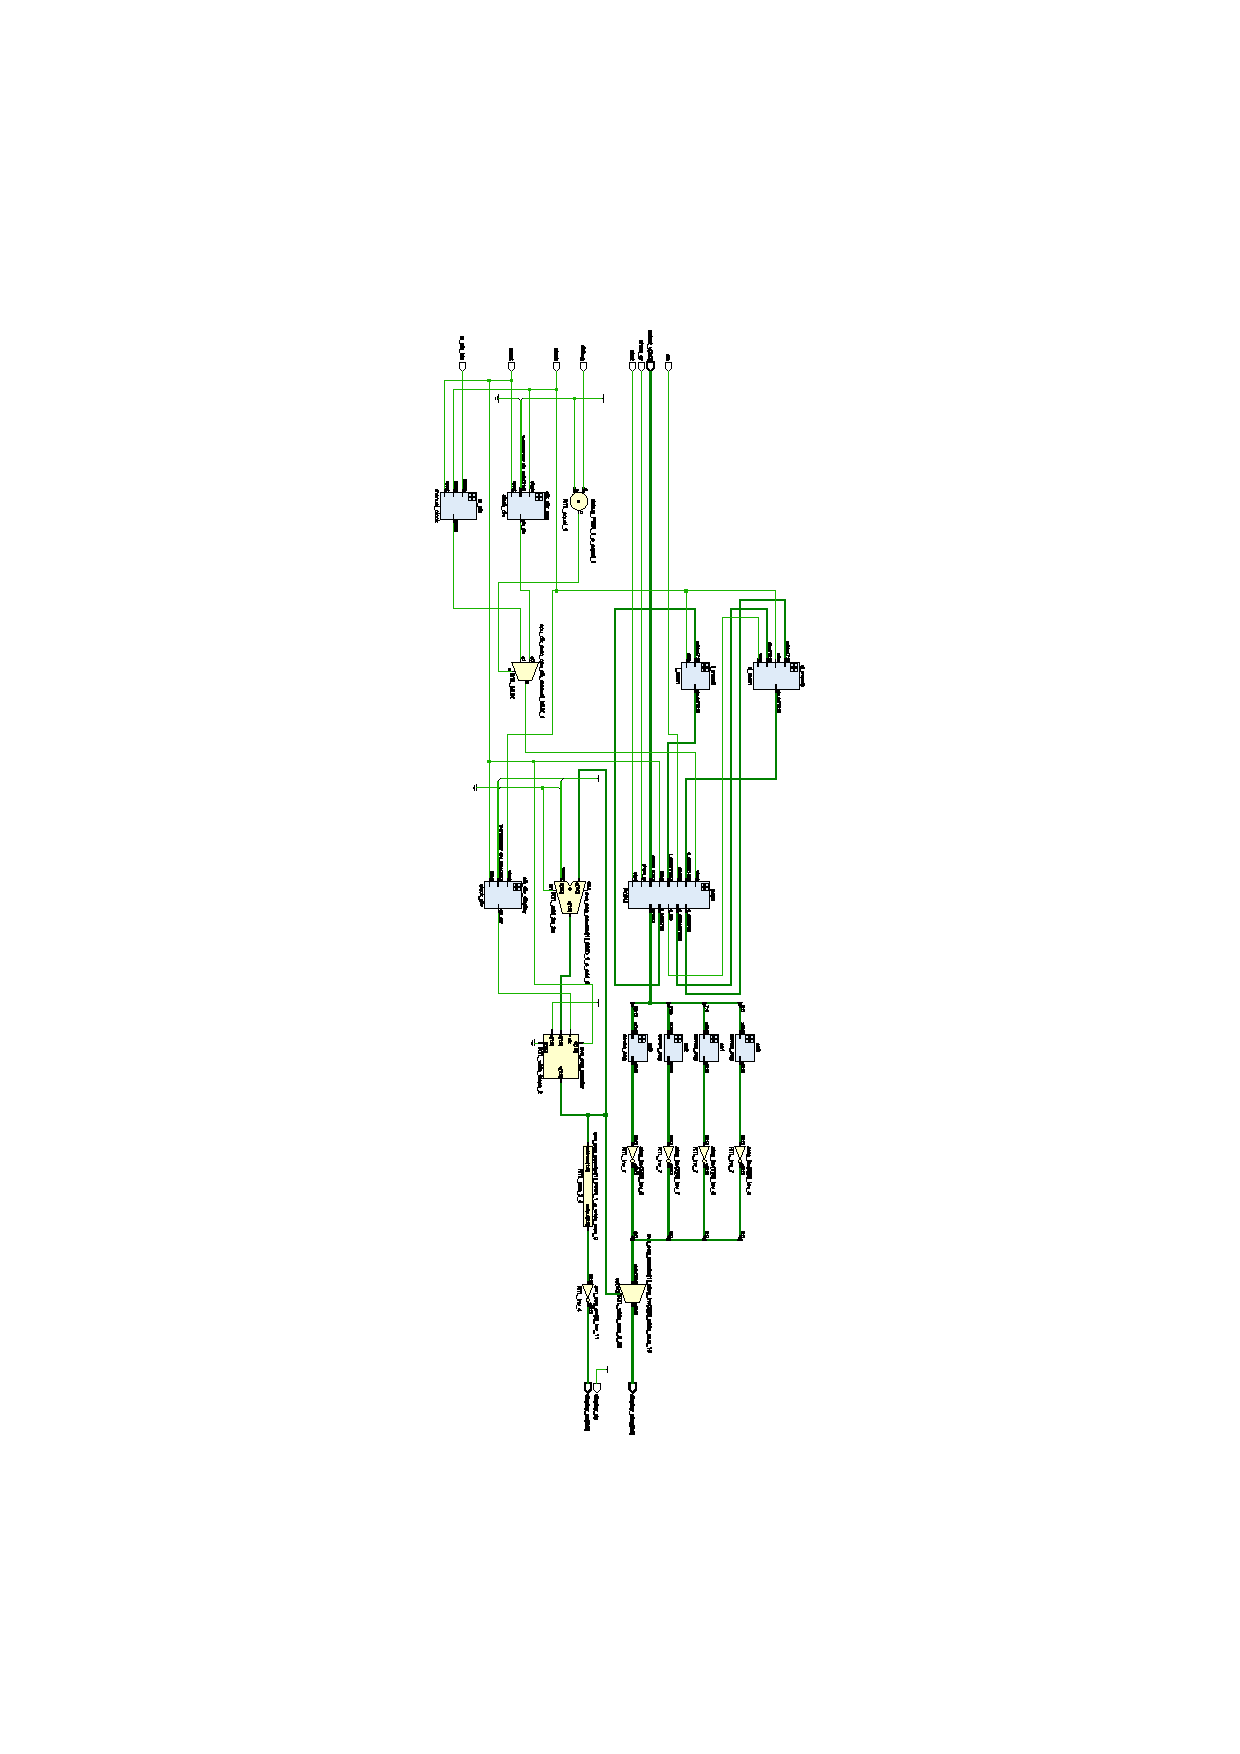
\includegraphics[width=0.65\textwidth]{figure/topex.pdf}
  \caption{顶层模块的RTL图(Xilinx PlanAhead 14.7导出)}
\end{figure}
\newpage
\thispagestyle{empty}
\vspace{-2cm}
\begin{figure}[H]
  \hspace{-2cm}
  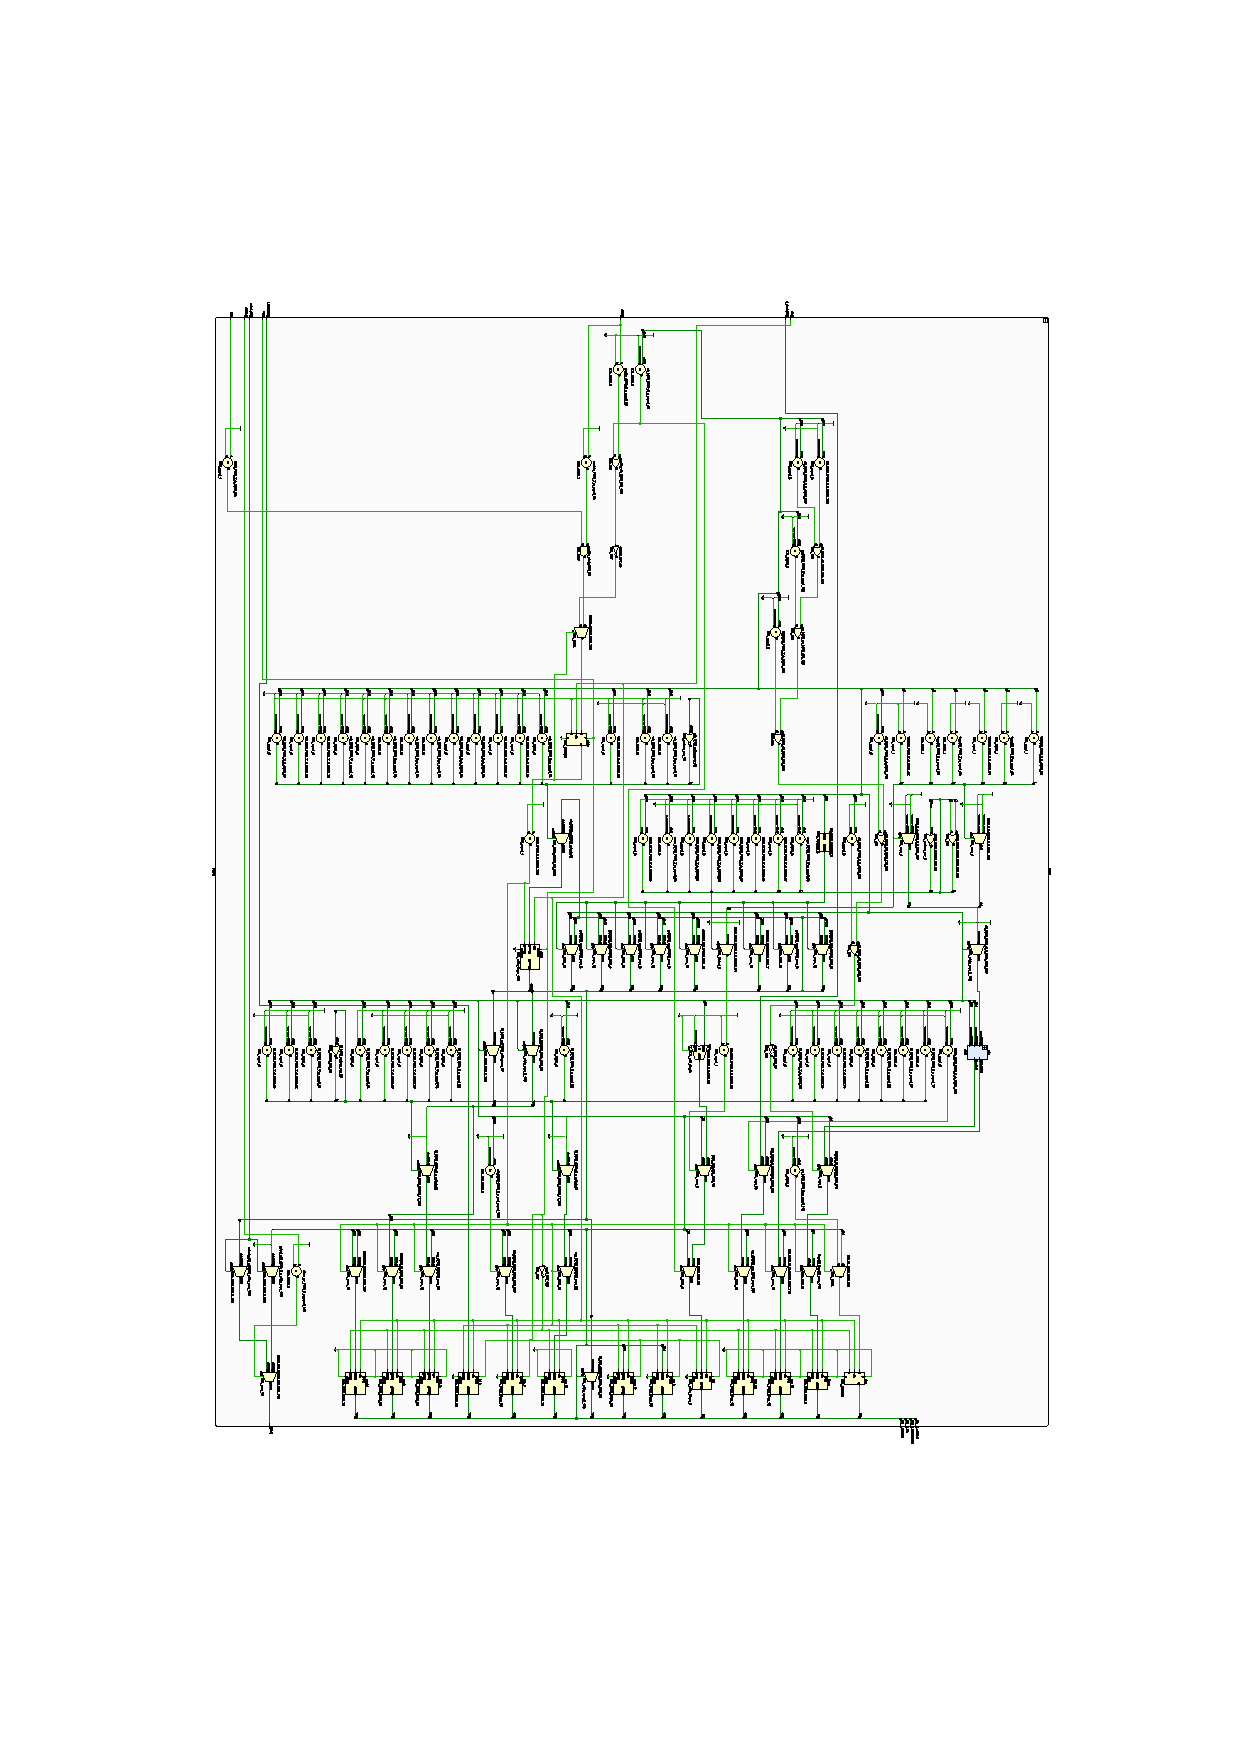
\includegraphics[width=1.2\textwidth]{figure/pcpuex.pdf}
  \caption{PCPU模块的RTL图(Xilinx PlanAhead 14.7导出)}
\end{figure}
\newpage
\section{实验设计代码}
header.v
\lstinputlisting{code/header.v}
\par top.v
\lstinputlisting{code/top.v}
\par manual\_clock.v
\lstinputlisting{code/manual_clock.v}
\par PCPU.v
\lstinputlisting{code/PCPU.v}
\par ALU.v
\lstinputlisting{code/ALU.v}
\par pcpu\_tb.v
\lstinputlisting{code/pcpu_tb.v}
\par pin.ucf
\lstinputlisting[language=bash,morekeywords={NET,LOC}]{code/pin.ucf}
\section{其他代码及脚本}
\par 文件目录
\dirtree{%
      .1 {\bf tools}.
      .2 {\bf assembler}.
      .3 opcode.h .
      .3 expression.h .
      .3 assembler.cpp .
      .2 {\bf coe\_generator}.
      .3 gcoe.cpp .
      .2 {\bf mem}.
      .3 mem.cpp .
      .2 assembler.exe .
      .2 gcoe.exe .
      .2 mem.exe .
      .2 compilerall.bat .
      .2 makeicoe.bat .
      .2 makedcoe.bat .
      .2 code.asm .
      .2 def\_d\_mem.txt .
      .2 i\_mem.mif .
      .2 i\_mem.coe .
      .2 d\_mem.mif .
      .2 d\_mem.coe .
    }
\par opcode.h
\lstinputlisting[language=C++]{code/tools/assembler/opcode.h}
\par expression.h
\lstinputlisting[language=C++]{code/tools/assembler/expression.h}
\par assembler.cpp (partly)
\lstinputlisting[language=C++]{code/tools/assembler/assembler.cpp}
\par gcoe.cpp
\lstinputlisting[language=C++]{code/tools/coe_generator/gcoe.cpp}
\par mem.cpp
\lstinputlisting[language=C++]{code/tools/mem/mem.cpp}
\par def\_d\_mem.txt
\lstinputlisting[language=bash]{code/tools/def_d_mem.txt}
\par compileall.bat
\lstinputlisting[language=bash]{code/tools/compileall.bat}
\par makeicoe.bat
\lstinputlisting[language=bash]{code/tools/makeicoe.bat}
\par makedcoe.bat
\lstinputlisting[language=bash]{code/tools/makedcoe.bat}
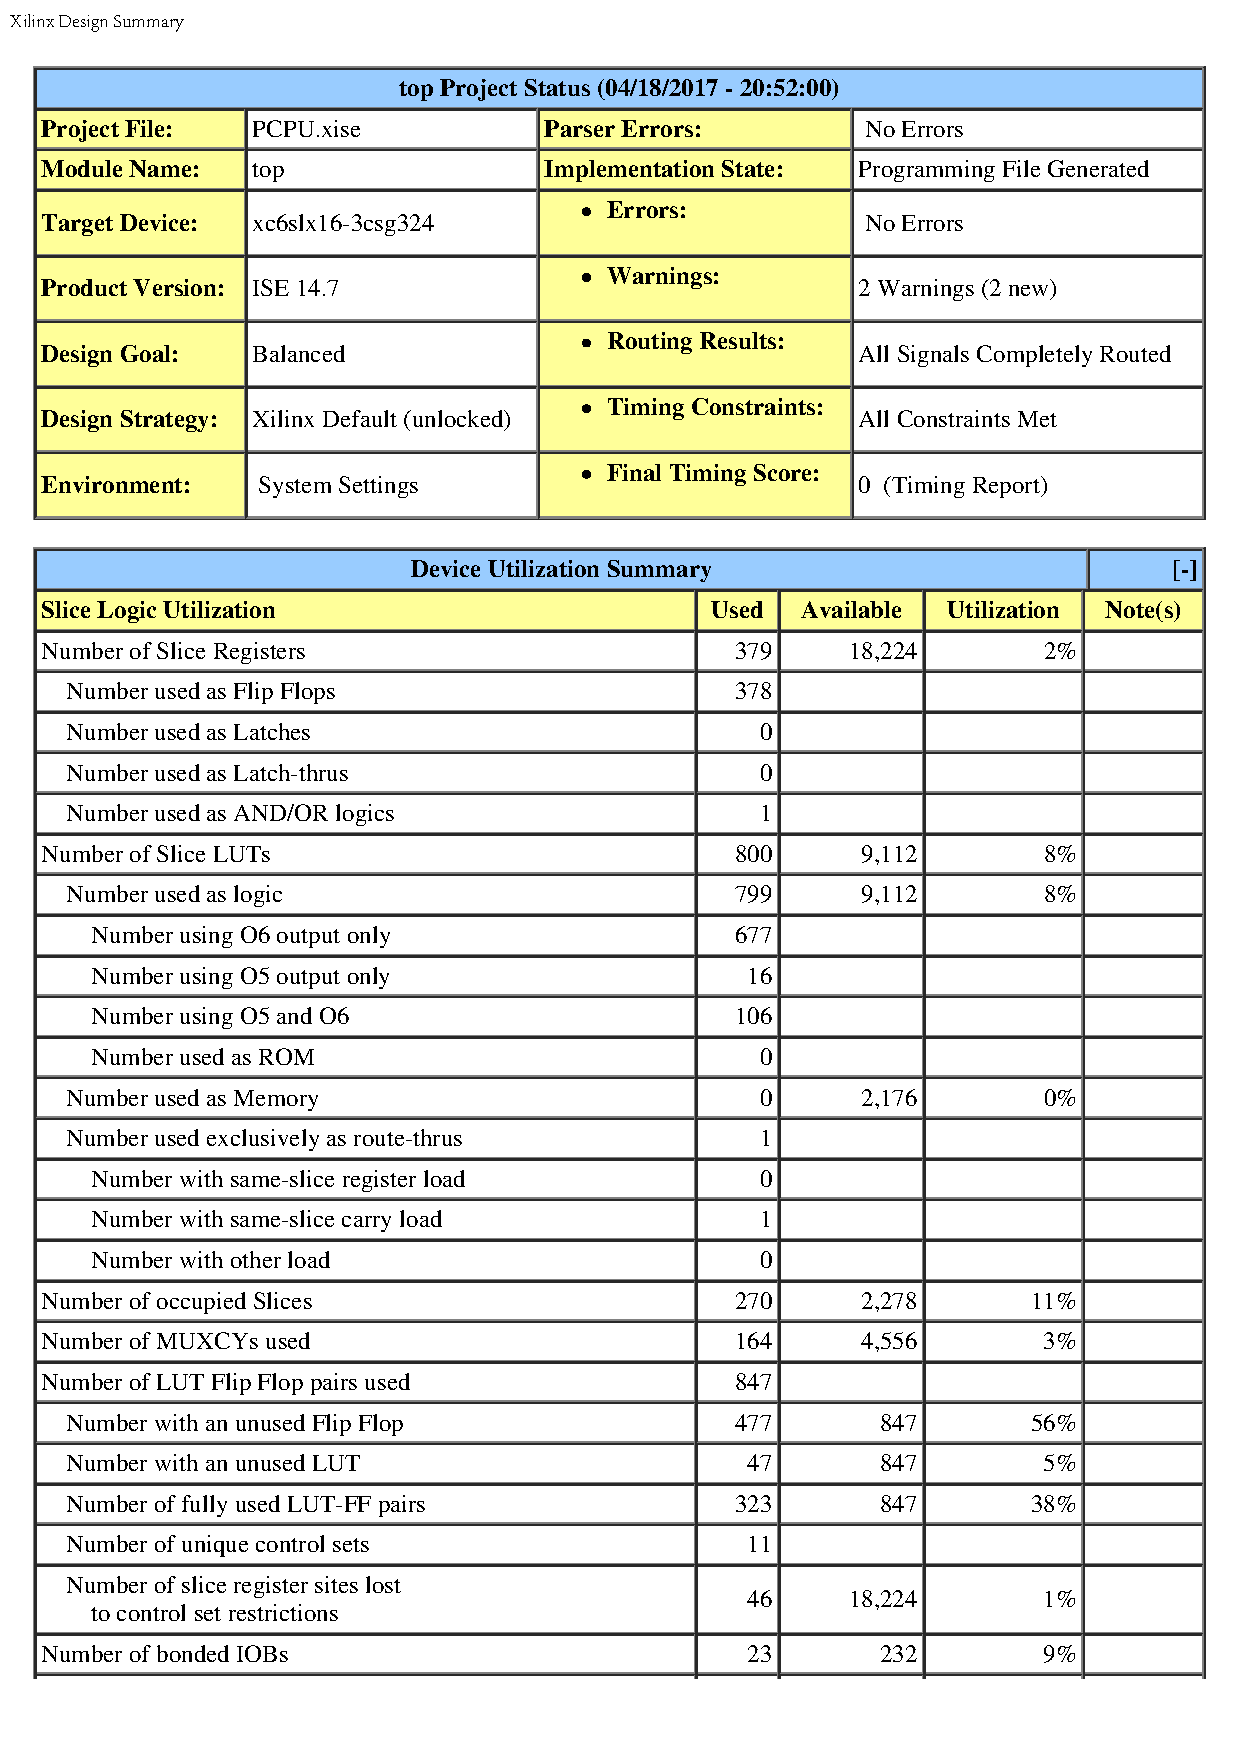
\includepdf[pages=1-2]{top_summary.pdf}
\end{document}
